%% SOICT 2026 submission -- Springer CCIS / LNCS (llncs.cls).
%% 12 pages excluding references; single blind (authors shown); no page numbers.
%% CAMERA-READY: delete the two \pagestyle/\thispagestyle{empty} lines.

\documentclass[runningheads,a4paper]{llncs}

\usepackage[T1]{fontenc}
\usepackage[utf8]{inputenc}
\usepackage{amsmath}
\usepackage{amssymb}
\usepackage{booktabs}
\usepackage{array}
\usepackage{graphicx}
\usepackage{tikz}
\usepackage[hidelinks]{hyperref}

\setlength{\emergencystretch}{1.5em}

\begin{document}
\pagestyle{empty}

\title{GUIStep: A Compact Vision--Language Model for\\
GUI Step Instruction Generation}

\titlerunning{GUIStep}

\author{Le Doan Phuong Uyen\inst{1} \and Nguyen Hong Buu Long\inst{1}}

\authorrunning{L. D. P. Uyen and N. H. B. Long}

\institute{Faculty of Information Technology, University of Science, VNU-HCM,\\
Ho Chi Minh City, Vietnam\\
\email{24C15039@student.hcmus.edu.vn}, \email{nhblong@fit.hcmus.edu.vn}}

\maketitle
\thispagestyle{empty}

\begin{abstract}
Most GUI agents map a screenshot and a goal to an action coordinate. We study the complementary
task of generating a sentence that tells a person which element to touch next, and we present
GUIStep, a compact vision--language model for it. Rather than collecting new annotations, we
reuse the human step instructions in AndroidControl and automatically derive structured target
declarations from the accessibility tree, which yields $64{,}567$ training examples. We compare
sentence-only QLoRA adaptation of Qwen2.5-VL-3B-Instruct with adaptation on a declaration followed
by the sentence, and we then refine the declaration model using preference pairs that differ in
the declared element. Since one element admits many valid descriptions, we evaluate the generated
sentence by \emph{execution}: a frozen grounding model maps it back to the screen, and the score
checks the recovered element together with the action class. On $4{,}463$ held-out touch steps,
our refined model reaches $66.5$ executability against $53.6$ for the untuned backbone, and
BLEU-4 rises from $15.3$ to $49.9$. The ablation, however, attributes most of that improvement to
sentence-only adaptation: the structured stages recover their added complexity but do not
significantly outperform it.
\keywords{GUI instruction generation \and vision--language model \and referring expression
\and mobile user interface}
\end{abstract}

%------------------------------------------------------------------------------
\section{Introduction}
\label{sec:intro}

A user who stops halfway through a phone task needs one sentence, such as \emph{Click on the
share icon at the top right of the screen}, written for a person rather than for a program.

Research on GUI agents usually targets a different output. Given a screenshot and a goal,
SeeClick~\cite{seeclick}, OS-Atlas~\cite{osatlas} and UGround~\cite{uground} emit a
machine-readable action such as \texttt{click(872,141)} so that software can act on the
user's behalf. Any language they produce along the way is an intermediate representation rather
than an output to be judged. Our target is instead the next-step instruction itself,
written for a human reader; Fig.~\ref{fig:overview} shows one such step.

\begin{figure}[t]
\centering
\begin{tikzpicture}[font=\footnotesize]
% screenshot node spans x in [0,3.3], y in [-3.373,0]; touch at 14.2% width, 33.2% height
\node[anchor=south west,text width=11.7cm,align=left,inner sep=0pt] at (0,0.2)
  {\textbf{Goal.} I travel with Aer Lingus Airlines regularly and like their service, so look up
  the flight details in the booking.com app and sort by the cheapest direct flight\\[2pt]
  \textbf{Previous steps.} Click on the airlines option at the top of the screen $\rightarrow$
  Click on Aer Lingus option $\rightarrow$ Click on done option};
\node[inner sep=0pt,anchor=north west] (img) at (0,0)
  {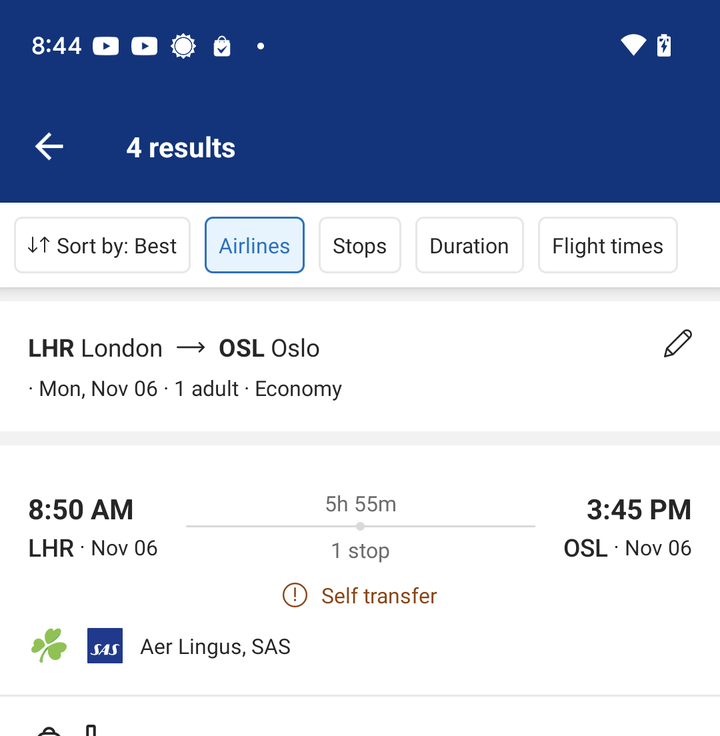
\includegraphics[width=3.3cm]{fig1_screen.png}};
\draw[red!70!black,line width=0.6pt] (0.468,-1.121) circle (2.9mm);
\fill[red!70!black] (0.468,-1.121) circle (0.3mm);
\node[draw,rounded corners,fill=black!6,anchor=west,align=center,
      minimum width=2cm,minimum height=0.9cm] (mod) at (3.9,-1.687)
  {GUIStep\\[-1pt]{\scriptsize (Sect.~\ref{sec:model})}};
\node[anchor=west,text width=5.2cm,align=left] (out) at (6.5,-1.687)
  {\textbf{generated:} \emph{``Click on the sort by option''}};
\node[anchor=north west,text width=5.2cm,align=left] at (6.48,-2.0)
  {\textbf{reference:} \emph{``Click on sort by option at the top left of the screen''}};
\draw[->,thick] (3.45,-1.687) -- (3.85,-1.687);
\draw[->,thick] (5.95,-1.687) -- (6.4,-1.687);
\end{tikzpicture}
\caption{One step of the task, from a held-out episode of
AndroidControl~\cite{androidcontrol}. The OCR strings the model also reads are omitted. Five filter
chips compete on this screen, so the instruction has to name the intended one. The circle marks the
recorded touch and is not shown to the model.}
\label{fig:overview}
\end{figure}

GUIStep reuses AndroidControl's human step instructions and constructs the remaining supervision
by rule~\cite{androidcontrol}. Our two QLoRA~\cite{qlora} adaptations of
Qwen2.5-VL-3B-Instruct~\cite{qwen25vl} both start from the same backbone. The first predicts the
instruction directly, whereas the second predicts a structured declaration of the target element
before the instruction. A preference objective then refines the declaration model using pairs
that share an instruction but declare different elements. All of our adapted models improve on
the untuned backbone, both in executability and in the standard reference-overlap metrics.

Scoring such a model is the second difficulty, since the task has no established automatic
metric. A sentence cannot be judged against a single reference when the same button has many
valid names: \emph{Click on the search bar} and \emph{Tap the magnifying glass at the top} denote
one element, and no corpus lists the admissible wordings. Content-word string matching therefore
rejects $97.5\%$ of the valid rewordings we collected. Sentence-embedding similarity does no
better, reaching an AUC of only $0.336$ on $51$ hand-written cases. It measures topical
proximity rather than reference: \texttt{inbox}/\texttt{outbox} scores $0.76$, while
\texttt{search}/\texttt{magnifying glass}, the pair that denotes one button, scores $0.55$.

We therefore adopt the criterion used in referring expression generation, where a description is
adequate if a \emph{listener} recovers the referent~\cite{mao2016,luo2017,yu2016}. On phone
screens our listener is a frozen grounding model that reads the sentence and returns a point, and
we call the resulting score \emph{executability}. The listener is itself a learned model, so we
first validate its localisation, its sensitivity to paraphrase and its dependence on its own
training data. Reference instructions reach $83.8$ under this score, and we interpret all
results against that measured ceiling rather than against $100$.

Our main contributions are as follows.
\begin{itemize}
\item \textbf{GUIStep, an automatically constructed training pipeline for GUI step instruction
generation.} We reuse AndroidControl's instructions, derive target declarations from the
accessibility tree and construct preference pairs from competing elements, all without collecting
additional labels (Sects.~\ref{sec:data}--\ref{sec:model}).
\item \textbf{An execution-based score for the generated instructions.} A frozen listener maps
each instruction back to the screen, and the score checks the recovered element together with the
action class. We also measure the ceiling, the floor, the robustness to paraphrase and the
dependence on the chosen listener (Sect.~\ref{sec:metric}).
\end{itemize}

%------------------------------------------------------------------------------
\section{Related Work}
\label{sec:related}

\paragraph{Language about graphical interfaces.}
Widget Captioning~\cite{widgetcap} describes a UI element that has already been selected
and names visually identical widgets as its hard case; Screen2Words~\cite{screen2words} summarises
a whole screen. VUT~\cite{vut}
shares one encoder across five UI tasks, while Spotlight~\cite{spotlight} and
Ferret-UI~\cite{ferretui} work from pixels with a region of focus. In contrast, our task does not
supply the target element, so the model must select the next
step before it can describe it. Each
step also carries one reference rather than five, which is why we treat CIDEr-D as comparable
only across the rows of our own experiment.

\paragraph{GUI control and grounding.}
AndroidControl~\cite{androidcontrol} records $15{,}283$ human episodes and uses each step's
instruction as \emph{input} to action prediction, whereas we use it as the generation target and
take our localisation rule from its Appendix~D.3. Android-in-the-Wild~\cite{aitw} is the source
of the $0.14$ normalised tolerance that is widely used to judge a predicted coordinate, whose
cost we measure in Sect.~\ref{sec:rules} before adopting a rule. Grounding
models~\cite{seeclick,osatlas,uground} map an expression to a point; we use one as an
\emph{instrument} rather than as a system under test, and Sect.~\ref{sec:validate} reports its
measured error and its training composition.

\paragraph{Listener-based evaluation.}
That a description succeeds when a listener recovers the referent is due to the discriminative
line in referring expression generation~\cite{mao2016,luo2017,yu2016}. Newman et
al.~\cite{newman2020} show that a model listener tracks communicative success
better than $n$-gram overlap, and Zhao et al.~\cite{zhao2021} reach a compatible conclusion for
navigation instructions; they also print a human reference beside system scores, the presentation
we adopt. Validating a metric with error injections and thresholds published in advance follows
Sai et al.~\cite{sai2021}. Prior work also cautions that automatic proxies may diverge from human
judgement~\cite{clark2021} and that GUI grounders can be brittle under
rephrasing~\cite{groundersunderstand}. Sect.~\ref{sec:validate} tests both concerns.

%------------------------------------------------------------------------------
\section{Task and Training Data}
\label{sec:data}

\paragraph{Task.}
At step $t$, the model receives a screenshot, the episode goal, the previous three reference step
instructions and up to $24$ OCR detections from the current screen. OCR strings are returned by
RapidOCR at confidence at least $0.5$ and retained in detector order. The model emits one English
sentence naming the next action and its target. The target box, recorded point, selected widget
and accessibility tree are not model inputs. Training includes all action types; evaluation uses
the $4{,}463$ touch steps for which a target point is available. A fixed prompt presents the goal,
history and OCR text in that order before requesting the next-step instruction.

\paragraph{Construction.}
We join the instruction mirror
\url{https://huggingface.co/datasets/HarrytheOrange/parsed_AndroidControl} with the image mirror
\url{https://huggingface.co/datasets/ckg/AndroidControlParsedWithImages-20k} on
\texttt{(episode\_id, step\_id)}. The supervised sentence target is AndroidControl's recorded
human instruction; the accessibility trees come from \texttt{all\_forest\_dict.zip} in the first
mirror. Keys missing from either mirror are dropped. As an alignment check, the
OCR text at the recorded touch overlaps the corresponding instruction on $48\%$ of $400$ sampled
steps, compared with $20\%$ after shifting the instruction by one step. The resulting corpus has
$64{,}567$ training steps over $12{,}895$ tasks and $6{,}958$ test steps over $1{,}432$ disjoint
tasks. Applications may occur in both partitions.

\paragraph{Scoring population and statistics.}
Scoring needs a recorded point, so the evaluation population is the $4{,}463$ test steps whose
action is a touch ($4{,}446$ taps and $17$ long presses). The $2{,}495$ non-touch steps
(\texttt{wait}, \texttt{open\_app} and similar) have no point to compare against and are
excluded, so all metrics are computed on the same population. Steps within an app are not
independent, so confidence intervals use $10{,}000$ cluster bootstrap resamples over
apps~\cite{cameron2008}, and paired comparisons use McNemar's test.

%------------------------------------------------------------------------------
\section{GUIStep}
\label{sec:model}

All three configurations of GUIStep adapt Qwen2.5-VL-3B-Instruct~\cite{qwen25vl} with 4-bit NF4
QLoRA~\cite{lora,qlora} under LLaMA-Factory~\cite{llamafactory}: rank $8$, scale $16$, dropout
$0.05$, adapters on the seven decoder projections, frozen vision tower and multimodal projector,
and context length $2{,}560$. We apply the loss to assistant tokens only and decode greedily.
Two of the configurations start independently from the backbone, and the third continues from the
second, so they do not form a single sequential pipeline.

\paragraph{GUIStep-S: sentence-only adaptation.}
This configuration starts from the pretrained backbone and uses the recorded step instruction as
its training target. Training runs for two epochs ($8{,}072$ updates), with effective batch $16$,
peak learning rate $10^{-4}$, cosine decay and $5\%$ warm-up.

\paragraph{GUIStep-D: declaration adaptation.}
The second configuration also starts from the pretrained backbone and follows the same SFT
schedule, except that touch targets now begin with a structured declaration:
\begin{center}
\texttt{<desc>role | name | <point>x,y</point> | relation</desc>}
\end{center}
Here the target node is the smallest visible accessibility node containing the recorded touch.
Its role comes from a fixed map over Android classes that yields eleven interaction roles such as
\texttt{button}, \texttt{tappable text}, \texttt{text field} and \texttt{switch}, with container
classes mapping to \texttt{item} and the remainder to \texttt{element}. The name is the first
valid accessibility \texttt{text} or \texttt{content\_description}; otherwise we use the first one
or two OCR strings inside the node in top-to-bottom, left-to-right order. The point is the recorded
touch normalised to a $0$--$1000$ grid. The relation uses the nearest OCR string whose centre is
outside the node and within $350$ native-image pixels, expressed as above, below, left or right.
If no such string exists, a fixed template states whether the role is unique or gives its
same-role count. Non-touch steps retain the sentence target without a declaration. For example:
\begin{center}
\texttt{<desc>item | Close | <point>274,285</point> | just below ``3:09''</desc>}
\end{center}

\paragraph{GUIStep-P: preference refinement.}
Our third configuration continues from the GUIStep-D adapter. For each touch step we first select
the nearest visible node with the same role, excluding the target itself and any node nested in it
or overlapping more than half of the smaller node. We retain the resulting pair if the two names
and points differ and the centre distance falls between $80$ and $350$ native-image pixels. The
preferred output carries the target declaration, the rejected output carries this competing
declaration, and both end with the same recorded instruction, so the two sides differ only in the
element they name. This procedure yields $22{,}854$ pairs, on which we train with
ORPO~\cite{orpo} ($\beta=0.1$) for $800$ updates at learning rate $2\times10^{-5}$. That step
also adds training compute, however, so we run a matched control that applies cross-entropy to
the preferred outputs alone, for the same steps and the same number of updates.

\paragraph{Evaluated output.}
We store the declaration target as \texttt{<desc>...\allowbreak</desc>}, a newline and the
recorded instruction. GUIStep-S is thus scored directly, whereas for GUIStep-D and
GUIStep-P we remove the first generated declaration and score the first line that follows; a
declaration without a closing tag yields an empty instruction and consequently a failed step.
The evaluation listener does not receive the declaration.

%------------------------------------------------------------------------------
\section{Evaluation Metric}
\label{sec:metric}

\subsection{Definition}

Let $s$ be the generated sentence, $I$ the screenshot, $g$ the recorded touch and $B(g)$ the
bounding box of the element that was touched. Let $G$ be a grounding model that is independent of
the system under test, kept frozen and given no access to $g$, so that $p=G(I,s)$. A step counts
as correct when three conditions hold jointly.

\begin{description}
\item[(i) Action class.] The normalised action class of $s$ matches that of the reference. Twelve
surface verbs (\emph{tap, click, press, select, choose, touch, open, launch, go, navigate, visit,
view}) collapse into one touch class, since on screen each denotes one contact; the five classes
kept apart are touch, type, scroll, long press and back.
\item[(ii) No polarity inversion.] $s$ and the reference must not name opposite states of one
control, since \emph{enable notifications} and \emph{disable notifications} share a touch point;
the check uses a hand-written table of nine pairs.
\item[(iii) Localisation.] $p$ lies inside $B(g)$, the rule of AndroidControl's
Appendix~D.3~\cite{androidcontrol}:
\begin{equation}
p \in B(g) .
\label{eq:d3}
\end{equation}
\end{description}

Condition (iii) is strict: the median target covers $1.0\%$ of the screen, compared with $7.8\%$
for the $\pm14\%$ tolerance window of Android-in-the-Wild~\cite{aitw}. Fifteen steps whose
element carries no box count as failures.

\subsection{Choice of Localisation Rule}
\label{sec:rules}

Three localisation rules were available to us, and they disagree by up to $9$ points on the same
sentences. We chose between them by measuring both ends of each. First, the tolerance
window is the field's convention. Second, the in-box rule is Eq.~\ref{eq:d3}. Third and
strictest, the Voronoi rule requires $p$ to be closer to $g$ than to any other element centre.
Table~\ref{tab:rules} scores all three on one random slice of $800$ steps.

\begin{table}[t]
\centering
\caption{Choosing the localisation rule. One random slice of $800$ steps, identical sentences
scored under each rule. The floor bounds what a system can earn without identifying anything;
the usable range is the difference between the two measured ends. We adopt the in-box rule.}
\label{tab:rules}
\begin{tabular}{lrrr}
\toprule
sentence given to the listener & in-box (D.3) & Voronoi & window $\pm14\%$\\
\midrule
reference instruction (ceiling) & $83.0$ & $74.9$ & $83.0$\\
\midrule
\emph{``Tap the button.''} & $14.1$ & $12.0$ & $20.5$\\
reference of a \emph{different} screen & $8.6$ & $6.1$ & $12.8$\\
element name deleted, position kept & $74.8$ & $68.0$ & $78.9$\\
\midrule
\textbf{usable range} & $\mathbf{68.9}$ & $62.9$ & $62.5$\\
\bottomrule
\end{tabular}
\end{table}

The in-box rule has the widest measured range, as it retains the reference ceiling while keeping
the contentless floor below that of the tolerance window, and we adopt it as our primary score.
AndroidControl does not distribute target boxes for every step, however, so we
reconstruct each box as the smallest visible accessibility node containing the recorded touch.

%------------------------------------------------------------------------------
\subsection{Validation of the Metric}
\label{sec:validate}

Because executability depends on a learned listener, we validate the listener before we use it.
Table~\ref{tab:valid} summarises the checks, whose thresholds were all fixed before the
corresponding measurement was run.

\begin{table}[t]
\centering
\caption{Validation of the instrument. Thresholds in the second column were fixed before the
corresponding measurement was executed. Two of the ten error-injection criteria fail.}
\label{tab:valid}
\setlength{\tabcolsep}{4pt}
\begin{tabular}{p{4.6cm}p{1.7cm}p{3.3cm}l}
\toprule
check & threshold & measured & verdict\\
\midrule
median localisation error of the instrument & $\le 3\%$ of width & $0.7\%$ ($n=300$) & pass\\
false rejection of paraphrases & $\le 10\%$ & $0.0\%$ ($n=398$) & pass\\
false rejection under the action check & $\le 15\%$ & $0.0\%$ ($n=398$) & pass\\
catching a distant wrong element & $\ge 90\%$ & $99.6\%$ ($n=233$) & pass\\
catching a wrong action class & $\ge 80\%$ & $100.0\%$ ($n=369$) & pass\\
catching wrong content & $\ge 90\%$ & $91.1\%$ ($n=494$) & pass\\
\textbf{catching a near-adjacent element} & $\ge 80\%$ & $33.1\%$ ($n=121$) & \textbf{fail}\\
\textbf{catching out-of-table negation} & $\ge 50\%$ & $20.0\%$ ($n=15$) & \textbf{fail}\\
\bottomrule
\end{tabular}
\end{table}

For the frozen listener UGround-V1-2B~\cite{uground}, reference instructions score $83.8$
$[82.5,85.1]$, whereas contentless text scores $14.1$ $[11.7,16.7]$. On the $193$ sentences that
contain both a name and a position clause, deleting the name costs $34.2$ points, compared with
$4.7$ for deleting the position, so the score is driven mainly by the element name. On the full
$800$-step slice of Table~\ref{tab:rules} the name-deletion effect is a smaller $8.2$ points,
because most sentences there contain no removable position clause. Across $1{,}139$
meaning-preserving rewrites, finally, the net change is $-0.09$ points $[-0.93,+0.79]$.

Overall the injection suite passes eight of the ten criteria, and it is weak on near-adjacent
elements and on negations absent from the polarity table. UGround has itself seen AndroidControl
training data, so we repeat our main comparison with UI-Venus-Ground-7B~\cite{uivenus}, which has
not. The gap between GUIStep-S and the untuned backbone then changes from $+11.14$ to $+11.02$,
retaining $99\%$ of its magnitude.

%------------------------------------------------------------------------------
\section{Experiments}
\label{sec:results}

\subsection{Main Results}

\begin{table}[t]
\centering
\caption{Executability on the same $4{,}463$ touch steps. Scores are interpreted against the
measured reference ceiling of $83.8$.}
\label{tab:main}
\begin{tabular}{lrr}
\toprule
system & executability & 95\% CI\\
\midrule
untuned backbone & $53.6$ & $[51.9,55.3]$\\
GUIStep-S (sentence only) & $65.5$ & $[63.8,67.2]$\\
GUIStep-D (declaration) & $63.6$ & $[61.9,65.4]$\\
GUIStep-D $+$ cross-entropy (control) & $66.0$ & $[64.3,67.7]$\\
\textbf{GUIStep-P} (preference refined) & $\mathbf{66.5}$ & $[64.9,68.2]$\\
\midrule
reference instruction & $83.8$ & $[82.5,85.1]$\\
\bottomrule
\end{tabular}
\end{table}

Table~\ref{tab:main} reports executability for every configuration. GUIStep-P raises the score
from $53.6$ to $66.5$, a paired difference of $+13.0$ points $[+11.5,+14.4]$ ($p<0.001$).
Relative to the measured reference ceiling it reaches $79.4\%$, compared with $63.9\%$ for the
untuned backbone.

\subsection{Ablation}

The same table separates our three configurations, and the picture it gives is more qualified.
GUIStep-D scores $1.9$ points below GUIStep-S $[-3.0,-0.7]$, so the structured target costs
accuracy on its own. GUIStep-P recovers that loss, but its $+1.05$-point difference from
GUIStep-S is not significant ($p=0.078$). Against the matched cross-entropy control, moreover,
the preference objective adds only $+0.52$ points $[+0.02,+1.00]$, which suggests that part of
the recovery comes from the extra updates rather than from the objective. Overall we attribute
the main gain to sentence-only adaptation: neither the structured target nor the preference
objective yields a clear improvement beyond it.

\subsection{Reference-Overlap Metrics}
For comparability with Widget Captioning and Screen2Words we also report the conventional
generation metrics in Table~\ref{tab:text}. We compute them at corpus level with the official
COCO Captions scorers after PTB tokenisation; chrF uses SacreBLEU, and BERTScore is
baseline-rescaled F1 from layer $17$ of \texttt{roberta-large}. Note that there is one reference
per step, which is why CIDEr-D exceeds $100$ and is comparable only between the rows of this
table.

\begin{table}[t]
\centering
\caption{Reference-overlap metrics on the same $4{,}463$ steps, one reference per step.}
\label{tab:text}
\setlength{\tabcolsep}{3.6pt}
\begin{tabular}{lrrrrrrr}
\toprule
& BLEU-4 & METEOR & ROUGE-L & CIDEr-D & SPICE & chrF & BERTScore\\
\midrule
untuned backbone & $15.3$ & $24.6$ & $42.3$ & $88.0$ & $18.5$ & $40.2$ & $40.1$\\
GUIStep-S & $51.6$ & $36.8$ & $67.3$ & $416.1$ & $\mathbf{44.4}$ & $61.3$ & $66.3$\\
GUIStep-D & $48.7$ & $35.8$ & $66.0$ & $387.7$ & $41.3$ & $59.9$ & $65.1$\\
GUIStep-P & $49.9$ & $\mathbf{37.3}$ & $\mathbf{68.5}$ & $401.0$ & $42.2$ & $\mathbf{61.8}$ &
$\mathbf{66.7}$\\
\midrule
reference & $100.0$ & $100.0$ & $100.0$ & $988.7$ & $98.6$ & $100.0$ & $100.0$\\
\bottomrule
\end{tabular}
\end{table}

All seven metrics improve substantially over the untuned backbone. Our configurations are ranked
differently here, however: GUIStep-S leads on BLEU-4, CIDEr-D and SPICE, whereas GUIStep-P leads
on METEOR, ROUGE-L, chrF and BERTScore. None of these metrics can tell whether the sentence
identifies the intended element. We read them as a complement to executability rather than as a
substitute for it.

\subsection{Error Analysis}
\label{sec:analysis}

GUIStep-P fails on $1{,}493$ steps. Only $50$ of those failures use the wrong action class,
while the other $1{,}443$ ($96.7\%$) describe the wrong element.
Typical examples are \texttt{select minutes 00} for \emph{click on the OK option} and
\texttt{Click on the Air India flight option} for \emph{Click on the Sort filter}. The main
remaining problem is thus element naming rather than action selection or fluency, which is
consistent with the hard case that Widget Captioning reports for visually identical
widgets~\cite{widgetcap}.

%------------------------------------------------------------------------------
\section{Limitations}
\label{sec:limits}

Our error-injection suite was run with the Voronoi localisation rule, whereas the primary score
uses the in-box rule. Since the in-box rule is the more permissive of the two, the detection
rates in Table~\ref{tab:valid} should be read as upper bounds. The reconstructed boxes are also
stricter than AndroidControl's original labels and are not directly comparable with them.

Executability remains a model-based proxy for whether a person can follow an instruction, and we
have not yet established that link with a human study. Our experiments also cover one English
corpus, one backbone and touch actions only, and they compare against the untuned backbone and our
matched controls rather than against an external generation system. Absolute levels are
conditional on UGround, because the independent listener cross-check covers the gap between the
backbone and our adapted models rather than every reported level. Finally, $17.3\%$ of the test
reference sentences occur verbatim in training, and the history we supply contains reference
instructions rather than the model's own previous outputs.

%------------------------------------------------------------------------------
\section{Conclusion}
\label{sec:conclusion}

We introduced GUIStep, a training framework for GUI step instruction generation that reuses
AndroidControl's human instructions and automatically derives declarations and preference pairs,
together with an execution-based score that we validated before use. GUIStep-P outperforms the
untuned backbone by $13.0$ points, although our ablation attributes most of that gain to
sentence-only adaptation, with neither the structured target nor the preference objective
improving clearly on it. One explanation is that our preference signal acts on the declaration
rather than on the sentence that is actually scored. Future work should therefore put the
grounding signal directly on the generated sentence, either by reranking sampled candidates or by
sequence-level training with a listener reward~\cite{scst,luodisc}, and should validate the
metric against human judgements.

%------------------------------------------------------------------------------
\begin{thebibliography}{99}

\bibitem{androidcontrol}
Li, W., Bishop, W.E., Li, A., Rawles, C., Campbell-Ajala, F., Tyamagundlu, D., Riva, O.:
On the effects of data scale on UI control agents. In: Advances in Neural Information Processing
Systems 37, Datasets and Benchmarks Track (2024)

\bibitem{aitw}
Rawles, C., Li, A., Rodriguez, D., Riva, O., Lillicrap, T.: Android in the Wild: a large-scale
dataset for Android device control. In: Advances in Neural Information Processing Systems 36,
Datasets and Benchmarks Track (2023)

\bibitem{seeclick}
Cheng, K., Sun, Q., Chu, Y., Xu, F., Li, Y., Zhang, J., Wu, Z.: SeeClick: harnessing GUI
grounding for advanced visual GUI agents. In: Proceedings of the 62nd Annual Meeting of the
Association for Computational Linguistics (2024)

\bibitem{osatlas}
Wu, Z., Wu, Z., Xu, F., Wang, Y., Sun, Q., Jia, C., Cheng, K., Ding, Z., Chen, L., Liang, P.P.,
Qiao, Y.: OS-ATLAS: a foundation action model for generalist GUI agents. In: International
Conference on Learning Representations (2025)

\bibitem{uground}
Gou, B., Wang, R., Zheng, B., Xie, Y., Chang, C., Shu, Y., Sun, H., Su, Y.: Navigating the
digital world as humans do: universal visual grounding for GUI agents. In: International
Conference on Learning Representations (2025)

\bibitem{uivenus}
Gu, Z., et al.: UI-Venus technical report: building high-performance UI agents with RFT.
arXiv:2508.10833 (2025), preprint

\bibitem{widgetcap}
Li, Y., Li, G., He, L., Zheng, J., Li, H., Guan, Z.: Widget captioning: generating natural
language description for mobile user interface elements. In: Proceedings of the 2020 Conference
on Empirical Methods in Natural Language Processing, pp. 5495--5510 (2020)

\bibitem{screen2words}
Wang, B., Li, G., Zhou, X., Chen, Z., Grossman, T., Li, Y.: Screen2Words: automatic mobile UI
summarization with multimodal learning. In: Proceedings of the 34th Annual ACM Symposium on User
Interface Software and Technology, pp. 498--510 (2021)

\bibitem{vut}
Li, Y., Li, G., Zhou, X., Dehghani, M., Gritsenko, A.: VUT: versatile UI transformer for
multi-modal multi-task user interface modeling. arXiv:2112.05692 (2021), preprint

\bibitem{spotlight}
Li, G., Li, Y.: Spotlight: mobile UI understanding using vision-language models with a focus.
In: International Conference on Learning Representations (2023)

\bibitem{ferretui}
You, K., Zhang, H., Schoop, E., Weers, F., Swearngin, A., Nichols, J., Yang, Y., Gan, Z.:
Ferret-UI: grounded mobile UI understanding with multimodal LLMs. In: European Conference on
Computer Vision, pp. 240--255 (2024)

\bibitem{mao2016}
Mao, J., Huang, J., Toshev, A., Camburu, O., Yuille, A., Murphy, K.: Generation and comprehension
of unambiguous object descriptions. In: IEEE Conference on Computer Vision and Pattern
Recognition, pp. 11--20 (2016)

\bibitem{luo2017}
Luo, R., Shakhnarovich, G.: Comprehension-guided referring expressions. In: IEEE Conference on
Computer Vision and Pattern Recognition, pp. 7102--7111 (2017)

\bibitem{yu2016}
Yu, L., Poirson, P., Yang, S., Berg, A.C., Berg, T.L.: Modeling context in referring expressions.
In: European Conference on Computer Vision, pp. 69--85 (2016)

\bibitem{scst}
Rennie, S.J., Marcheret, E., Mroueh, Y., Ross, J., Goel, V.: Self-critical sequence training for
image captioning. In: IEEE Conference on Computer Vision and Pattern Recognition,
pp. 7008--7024 (2017)

\bibitem{luodisc}
Luo, R., Price, B., Cohen, S., Shakhnarovich, G.: Discriminability objective for training
descriptive captions. In: IEEE Conference on Computer Vision and Pattern Recognition,
pp. 6964--6974 (2018)

\bibitem{orpo}
Hong, J., Lee, N., Thorne, J.: ORPO: monolithic preference optimization without reference model.
In: Proceedings of the 2024 Conference on Empirical Methods in Natural Language Processing,
pp. 11170--11189 (2024)

\bibitem{newman2020}
Newman, B., Cohn-Gordon, R., Potts, C.: Communication-based evaluation for natural language
generation. In: Proceedings of the Society for Computation in Linguistics, pp. 116--126 (2020)

\bibitem{zhao2021}
Zhao, M., Anderson, P., Jain, V., Wang, S., Ku, A., Baldridge, J., Ie, E.: On the evaluation of
vision-and-language navigation instructions. In: Proceedings of the 16th Conference of the
European Chapter of the Association for Computational Linguistics, pp. 1302--1316 (2021)

\bibitem{sai2021}
Sai, A.B., Dixit, T., Sheth, D.Y., Mohan, S., Khapra, M.M.: Perturbation CheckLists for evaluating
NLG evaluation metrics. In: Proceedings of the 2021 Conference on Empirical Methods in Natural
Language Processing, pp. 7219--7234 (2021)

\bibitem{clark2021}
Clark, E., August, T., Serrano, S., Haduong, N., Gururangan, S., Smith, N.A.: All that's `human'
is not gold: evaluating human evaluation of generated text. In: Proceedings of the 59th Annual
Meeting of the Association for Computational Linguistics, pp. 7282--7296 (2021)

\bibitem{groundersunderstand}
Jandial, S., et al.: On the robustness of GUI grounding models against language variation.
arXiv:2408.04744 (2024), preprint

\bibitem{cameron2008}
Cameron, A.C., Gelbach, J.B., Miller, D.L.: Bootstrap-based improvements for inference with
clustered errors. Review of Economics and Statistics \textbf{90}(3), 414--427 (2008)

\bibitem{qwen25vl}
Bai, S., et al.: Qwen2.5-VL technical report. arXiv:2502.13923 (2025), preprint

\bibitem{lora}
Hu, E.J., Shen, Y., Wallis, P., Allen-Zhu, Z., Li, Y., Wang, S., Wang, L., Chen, W.: LoRA:
low-rank adaptation of large language models. In: International Conference on Learning
Representations (2022)

\bibitem{qlora}
Dettmers, T., Pagnoni, A., Holtzman, A., Zettlemoyer, L.: QLoRA: efficient finetuning of quantized
LLMs. In: Advances in Neural Information Processing Systems 36 (2023)

\bibitem{llamafactory}
Zheng, Y., Zhang, R., Zhang, J., Ye, Y., Luo, Z., Feng, Z., Ma, Y.: LlamaFactory: unified efficient
fine-tuning of 100+ language models. In: Proceedings of the 62nd Annual Meeting of the Association
for Computational Linguistics, System Demonstrations, pp. 400--410 (2024)

\end{thebibliography}

\end{document}
